\documentclass[a4paper,11pt]{article}

\usepackage[left=2cm,text={17cm, 24cm},top=3cm]{geometry}
\usepackage[czech]{babel}
\usepackage[utf8]{inputenc}
\usepackage{times}
\usepackage{hyperref}

\usepackage{multicol}
\usepackage{multirow}
\usepackage[czech,ruled,linesnumbered]{algorithm2e}
\usepackage{graphicx}
\usepackage{pdflscape}
\usepackage{pict2e}
% \usepackage{}

\begin{document}

\thispagestyle{empty}
\begin{center}
    \Huge \textsc{Vysoké učení technické v Brně}\\
    \huge\textsc{Fakulta informačních technologií}\\
    
    \vspace{\stretch{0.382}}
    
    Typografie a publikování -– 3. projekt\\
    \textbf{Tabulky a obrázky}\\
    
    \vspace{\stretch{0.618}}
\end{center}

{\LARGE 31. března 2025 \hfill Smirnov Nikita (xsmirn02)}
\clearpage

\setcounter{page}{1}

\section{Úvodní strana}
Název práce umístěte do zlatého řezu a nezapomeňte uvést \textit{dnešní} (today) datum a vaše jméno a příjmení.

\section{Tabulky}
 Pro sázení tabulek můžeme použít buď prostředí \texttt{tabbing} nebo prostředí \texttt{tabular}.

\subsection{Prostředí \texttt{tabbing}}
Při použití \texttt{tabbing} vypadá tabulka následovně:

\begin{tabbing}
    Vodní melouny\quad \=  Množství\quad \= Jednotka\quad \= Cena za jedn.\quad \= \kill
    Ovoce \> Množství \> Jednotka \> Cena za jedn. \> Cena celková \\
    Jablka \> 3 \> kg \> 25,90 Kč \> 77,70 Kč \\
    Hrušky \> 2,5 \> kg \> 27,40 Kč \> 68,50 Kč \\
    Vodní melouny \> 1 \> kus \>  35,– Kč \> 35,– Kč \\
\end{tabbing}
Toto prostředí se dá také použít pro sázení algoritmů, ovšem vhodnější je použít prostředí \texttt{algorithm} nebo \texttt{algorithm2e} (viz sekce 3).

\subsection{Prostředí \texttt{tabular}}
Další možností, jak vytvořit tabulku, je použít prostředí \texttt{tabular}. Tabulky pak budou vypadat takto\footnote{Kdyby byl problém s \texttt{cline}, zkuste se podívat třeba sem: \url{http://www.abclinuxu.cz/tex/poradna/show/325037}}:

\vspace{1.5em}
\begin{table}[h]
    \catcode`\-=12 % fix na cline 
    \centering
    \begin{tabular}{|c|c|c|}
         \hline & \multicolumn{2}{c|}{\textbf{Cena}} \\ \cline{2-3}
         \textbf{Měna} & \textbf{nákup} & \textbf{prodej} \\ \hline
         EUR & 23,26 & 24,93 \\ 
         GBP & 29,56 & 29,83 \\ 
         USD & 22,27 & 23,12 \\ 
         \hline
    \end{tabular}
    \caption{Tabulka kurzů k dnešnímu dni}
    \label{tab:currency}
\end{table}

\vspace{1.5em}
\begin{table}[h]
    \catcode`\-=12 % fix na cline 
    \centering
    
    \begin{tabular}{|c|c|}
    \hline
        $A$ & $\neg A$  \\ \hline
        \textbf{P} & N \\ \hline
        \textbf{O} & O \\ \hline
        \textbf{X} & X \\ \hline
        \textbf{N} & P \\ \hline
    \end{tabular}
    \begin{tabular}{|c|c|c|c|c|c|}
    \hline
        \multicolumn{2}{|c|}{\multirow{2}{*}{$A \wedge B$}} & \multicolumn{4}{c|}{$B$}\\ \cline{3-6}
        \multicolumn{2}{|c|}{} %upper row shift
            & \textbf{P} & \textbf{O} & \textbf{X} & \textbf{N} \\ \hline
        \multirow{4}{*}{$A$} 
            & \textbf{P} & P & O & X & N \\ \cline{2-6}
        & \textbf{O} & O & O & N & N \\ \cline{2-6}
        & \textbf{X} & X & N & X & N \\ \cline{2-6}
        & \textbf{N} & N & N & N & N \\ \hline
    \end{tabular}
    \begin{tabular}{|c|c|c|c|c|c|}
    \hline
        \multicolumn{2}{|c|}{\multirow{2}{*}{$A \vee B$}} & \multicolumn{4}{c|}{$B$}\\ \cline{3-6}
        \multicolumn{2}{|c|}{} %upper row shift
            & \textbf{P} & \textbf{O} & \textbf{X} & \textbf{N} \\ \hline
        \multirow{4}{*}{$A$} 
            & \textbf{P} & P & P & P & P \\ \cline{2-6}
        & \textbf{O} & P & O & P & O \\ \cline{2-6}
        & \textbf{X} & P & P & X & X \\ \cline{2-6}
        & \textbf{N} & P & O & X & N \\ \hline
    \end{tabular}
    \begin{tabular}{|c|c|c|c|c|c|}
    \hline
        \multicolumn{2}{|c|}{\multirow{2}{*}{$A \rightarrow B$}} & \multicolumn{4}{c|}{$B$}\\ \cline{3-6}
        \multicolumn{2}{|c|}{} %upper row shift
            & \textbf{P} & \textbf{O} & \textbf{X} & \textbf{N} \\ \hline
        \multirow{4}{*}{$A$} 
            & \textbf{P} & P & O & X & N \\ \cline{2-6}
        & \textbf{O} & P & O & P & O \\ \cline{2-6}
        & \textbf{X} & P & P & X & X \\ \cline{2-6}
        & \textbf{N} & P & P & P & P \\ \hline
    \end{tabular}

    %Ve vzorku to bylo jako odstavec, ale caption asi bude lep+si
    \caption{Protože Kleeneho trojhodnotová logika už je „zastaralá“, uvádíme zde příklad čtyřhodnotové logiky}
    \label{tab:math}
\end{table}

\clearpage

\section{Algoritmy}
Pokud budeme chtít vysázet algoritmus, můžeme použít prostředí \texttt{algorithm}\footnote{\url{http://ftp.cstug.cz/pub/tex/CTAN/macros/latex/contrib/algorithms/algorithms.pdf}} nebo \texttt{algorithm2e}. Příklad použití prostředí \texttt{algorithm2e}\footnote{\url{http://ftp.cstug.cz/pub/tex/CTAN/macros/latex/contrib/algorithm2e/doc/algorithm2e.pdf}} viz Algoritmus 1.



\begin{algorithm}
    \SetAlgoNoLine  
    \caption{\textsc{FastSLAM}}
        \SetKwFor{For}{for}{do}{end\:for}
        \SetNlSty{}{}{:}
        \SetNlSkip{-1em}
        
        \KwIn{\:$(X_{t-1}, u_t, z_t)$}   
        \KwOut{\:$X_t$}
        \vspace{0.5em}
        
        \Indp $\overline{X_t} = X_t = 0$ \\
        \For{$k = 1 ~\emph{to}~ M$} {
            $x^{[k]}_t = \textit{sample\_motion\_model}(u_t,x^{[k]}_{t-1})$ \\
            $\omega_t^{[k]} = \textit{measurement\_model}(z_t,x^{[k]}_t,m_{t-1})$ \\
            $m_t^{[k]} = updated\_occupancy\_grid(z_t,x^{[k]}_t,m^{[k]}_{t-1})$ \\
            $\overline{X_t} = \overline{X_t} + \langle x_x^{[m]},\omega_t^{[m]}\rangle$ \\
        }
        \For{$k = 1 ~\emph{to}~ M$}{
            draw $i$ with probability $\approx \omega^{[i]}_t$ \\
            add $\langle x^{[k]}_x,m^{[k]}_t \rangle$ to $X_t$ \\
        }
        \Return $X_t$
\end{algorithm}

\section{Obrázky}
Do našich článků můžeme samozřejmě vkládat obrázky. Pokud je obrázkem fotografie, můžeme klidně použít bitmapový soubor. Pokud by to ale mělo být nějaké schéma nebo něco podobného, je dobrým zvykem takovýto obrázek vytvořit vektorově.
\begin{figure}[h]
    \centering
    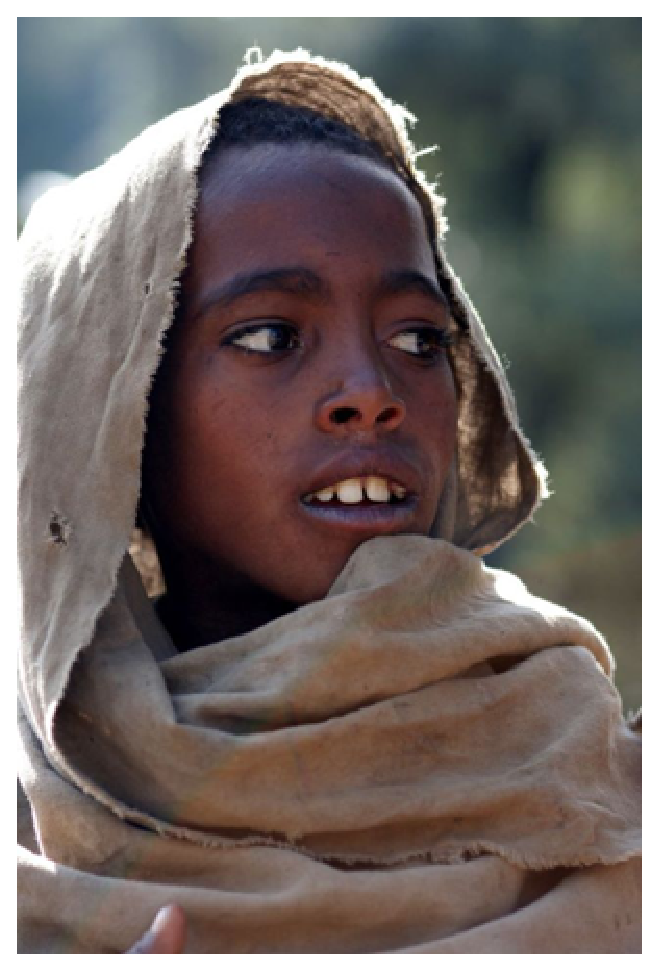
\includegraphics[width=0.25\linewidth]{etiopan.eps}
    \reflectbox{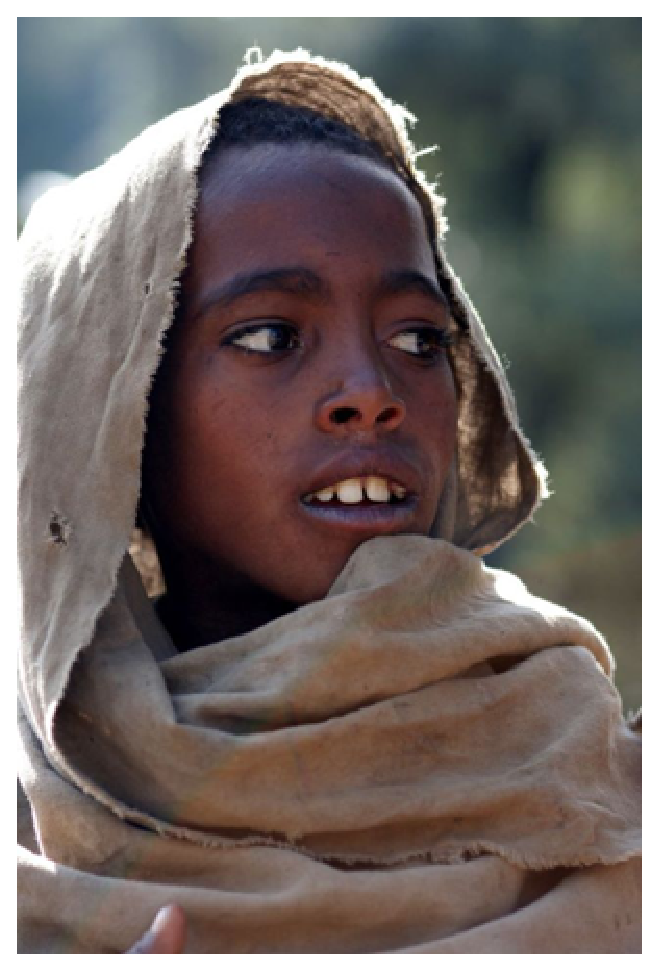
\includegraphics[width=0.25\linewidth]{etiopan.eps}}
    \caption{Malý Etiopánek a jeho bratříček}
    \label{fig:etiopanek}
\end{figure}

\clearpage

Rozdíl mezi vektorovým \dots 
\begin{figure}[h]
    \centering
    
\includegraphics[width=0.5\linewidth]{oniisan.eps}
    \caption{Vektorový obrázek}
    \label{fig:enter-label}
\end{figure}

\dots a bitmapovým obrázkem 
\begin{figure}[h]
    \centering
    
\includegraphics[width=0.5\linewidth]{oniisan2.eps}
    \caption{Bitmapový obrázek}
    \label{fig:enter-label}
\end{figure}

\noindent se projeví například při zvětšení. 

Odkazy (nejen ty) na obrázky 1, 2 a 3, na tabulky 1 a 2 a také na algoritmus 1 jsou udělány pomocí křížových odkazů. Pak je ovšem potřeba zdrojový soubor přeložit dvakrát.

Vektorové obrázky lze vytvořit i přímo v \LaTeX u, například pomocí prostředí \texttt{picture}.

% \clearpage

\begin{landscape}
    \begin{figure} [ht]
        \centering
        \setlength{\unitlength}{1mm}
        \begin{picture}(210, 120)
            \linethickness{1pt}
            \put(0,0){\framebox(210, 120){}}
            \put(30,20){\line(0,1){40}}
            \put(30,60){\line(1,0){40}}
            \put(70,54){\framebox(60, 12){}}%first rect
            \put(50,48){\framebox(140, 6){}}%second rect
            \put(60.5,35){\line(-10,12){10.6}}

            \put(130,57){\line(1,0){45}}
            \put(175,57){\line(0,-1){3}}
            
            \put(40,35){\line(1,0){40}}%stair top
            \put(40,20){\line(0,1){15}}
            \put(80,35){\line(5,-2){38}}

            \put(190,20){\line(0,1){10}} %pandus
            \put(190,30){\line(-1,0){97.5}}
            
            \put(187,30){\line(0,1){14}}
            \put(187,44){\line(-1,0){104}}
            \put(83,44){\line(0,-1){10}}

            \linethickness{0.1pt}
            \put(170, 90){\circle{20}}

            \linethickness{4pt}
            \put(10,20){\line(1,0){190}}
        \end{picture}

        %Kvůli tomu, že můj dům vypadá jako jednopodlažní krabice s okny.
        \caption{Vektorový obrázek moderního bydlení vhodného pro 21. století} 
        \label{fig:enter-label}
    \end{figure}
\end{landscape}

\end{document}
